\documentclass{article}

% if you need to pass options to natbib, use, e.g.:
%     \PassOptionsToPackage{numbers, compress}{natbib}
% before loading neurips_2018

% ready for submission
% \usepackage{neurips_2018}

% to compile a preprint version, e.g., for submission to arXiv, add add the
% [preprint] option:
%     \usepackage[preprint]{neurips_2018}

% to compile a camera-ready version, add the [final] option, e.g.:
     \usepackage[final]{neurips_2018}

% to avoid loading the natbib package, add option nonatbib:
 %   \usepackage[nonatbib]{neurips_2018}

\usepackage[utf8]{inputenc} % allow utf-8 input
\usepackage[T1]{fontenc}    % use 8-bit T1 fonts
\usepackage{hyperref}       % hyperlinks
\usepackage{url}            % simple URL typesetting
\usepackage{booktabs}       % professional-quality tables
\usepackage{amsfonts}       % blackboard math symbols
\usepackage{nicefrac}       % compact symbols for 1/2, etc.
\usepackage{microtype}      % microtypography
\usepackage{graphicx}
\usepackage{indentfirst}
\setlength{\parindent}{2em}
\usepackage{setspace}
\usepackage {subcaption}
\usepackage{float}
%\usepackage{subfigure}

\title{Quora Insincere Question Selection}
 
% The \author macro works with any number of authors. There are two commands
% used to separate the names and addresses of multiple authors: \And and \AND.
%
% Using \And between authors leaves it to LaTeX to determine where to break the
% lines. Using \AND forces a line break at that point. So, if LaTeX puts 3 of 4
% authors names on the first line, and the last on the second line, try using
% \AND instead of \And before the third author name.

\author{%
  Peihong Yu\quad  Xinru Zhang\quad Mengjie Min\\
  Stevens Institute Of Technology\\
  \texttt{pyu7@stevens.edu\quad
  	xzhan63@stevens.edu\quad
  	mmin@stevens.edu} \\
  % examples of more authors
  % \And
  % Coauthor \\
  % Affiliation \\
  % Address \\
  % \texttt{email} \\
  % \AND
  % Coauthor \\
  % Affiliation \\
  % Address \\
  % \texttt{email} \\
  % \And
  % Coauthor \\
  % Affiliation \\
  % Address \\
  % \texttt{email} \\
  % \And
  % Coauthor \\
  % Affiliation \\
  % Address \\
  % \texttt{email} \\
}

\begin{document}
% \nipsfinalcopy is no longer used

\maketitle
\begin{abstract}
	In this Kaggle competition, we aim at finding out inappropriate comments from Quora website by building a binary classification model. We separate our whole work into three steps. First, we use word embedding method to map each text into corresponding data. Second, we tried three different models to train the model. The approaches we adopt to solve the problem are "GRU", "LSTM" and "LSTM" nested “LSTM”. Finally the evaluation will base on the F1-score between the predicted score and the target score. Owing to the incorrect labels in datasets, the highest score in this competition is about 0.71. Our results is around 0.68 on the premise of  the datasets’ accuracy. Since attention model is so hot and has a high performance in NLP, we can try to adopt that tech to this deal with this problem. With paying more attention on parts of text, we may get a higher score using attention model.\\
\end{abstract}
\setlength{\parskip}{0.3em}
\section{Introduction}
\noindent Quora is a website for people to communicate with others. But sometimes inappropriate comments appear. Till now, the Quora has already implemented machine learning and hand-operated ways to decrease the possibility of insincere questions. In order to combat insincere questions more efficiency, help Quora maintain their policy with "Be Nice, Be Respectful". We need to find more up-gradable ways to discover these ambiguous and confusing comments.\\

\noindent Before introducing models, we want to clean the dataset first. If we feed our model with cleaner dataset, we can obtain a better result. Notice from the original data set, there are many disturbing characters. For the data pre-processing part, we majorly separate into three steps: \\

\indent1) Obtaining a dictionary by loading words from wiki-news-300d-1M.vec. \\
\indent2) Checking percentage of words from the training dataset also can found in "wiki" dataset.\\
\indent3) Discarding the punctuation, spaces and replace the misspell words into correct spell words.\\
\indent4) Selecting replaceable words in wiki datasets and replace the “cannot find” words with them.\\


\noindent Base on the organizer's command, we need to build a classifier to find out insincere questions. Dealing with the relationship with language, RNN is the general model we first think  to build our model. So our approach is motivated by the success of RNN model in natural language processing field. Firstly, we  use LSTM model, which is an improvement model of RNN. The LSTM model can choose some parts from the past can be kept and others can be forgotten, not like the general RNN model, selecting the most recent information without filtering. Furthermore, we also introduce GRU to build our model. Compared to LSTM, the commonality is that two models both keep the important information. The difference is that GRU model has fewer parameters than LSTM model, so the training speed is faster than LSTM.\\

\noindent In principle, by submitting results to kaggle, the highest score we got is 0.68421 and have a rank at 1055 among total 4037 groups , which is quite high at this point since the original dataset contains many wrong labels. At this time, the models we have are just simple LSTM, simple GRU and stack of LSTM and GRU. Attention will then be the next model we need to try in future work. The reason is that attention model will have the ability to focus on different parts of a text instead of putting more attention on useless words which may enhance the performance and increase accuracy.\\

\section{ Data Pre-processing}
\noindent The first and most important part of our project is data preprocessing.  We print the shape of training dataset and testing dataset on the first hand, the output shows that we have about 1306122 rows and 3 columns of data. The file train.csv has three columns: qid, question\_text, target. “Question\_text” column is composed of multiple sentences. “Target” column has binary values. “1” means that this sentence is identified as insincere. It will speed a lot of time running all the training dataset, so we choose to statistics the frequency of words and filter higher frequency of words to the next step.\\
\begin{figure}[h]
	\centering
	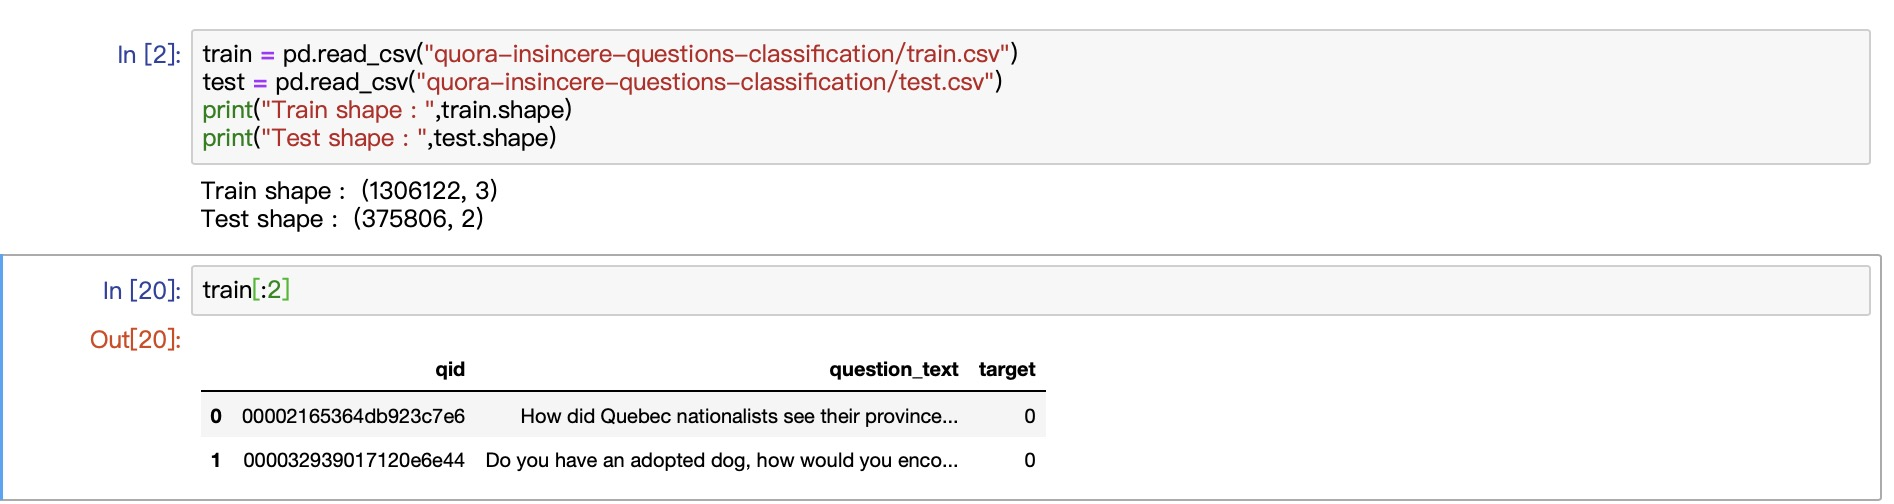
\includegraphics[scale = 0.15]{n1.jpeg}
	\caption{Information of training dataset
		}
\end{figure}\\
\noindent So how can we define whether a question is insincere or not? The key point is that we can capture some specific characters to decide the question is insincere. Thanks to the competition holder who generously provides us four datasets to help us with data processing part. We can use one of the datasets to match words so that we can judge is this word a good word or a bad word.\\

\noindent How we choose the high frequency words is that we build a dictionary named "vocab", each time the word appears from the training dataset, we add "1" to the value. Finally, we can add up totally numbers of each word. From the figure below, we 
enumerate the frequency of words in the first 5 rows.\\
\begin{figure}[h]
	\centering
	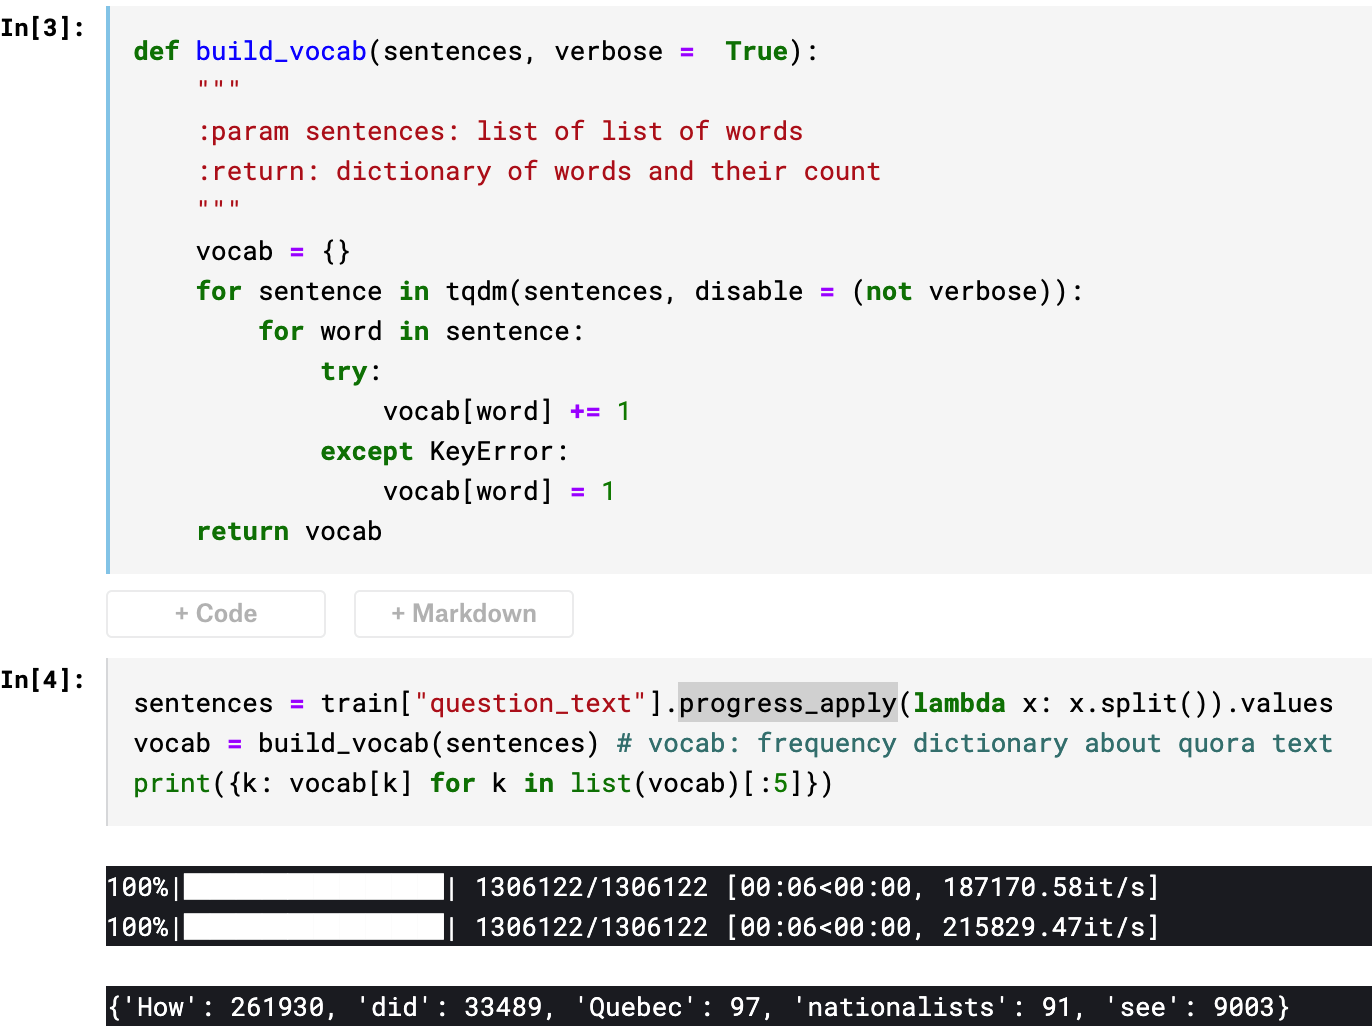
\includegraphics[scale = 0.15]{1.png}
	\caption{ First 10 rows of non-found words}
\end{figure}\\
\noindent As we can see on average questions in train and test datasets are similar, but there are quite long questions in train dataset.\\
\begin{figure}[h]
	\centering
	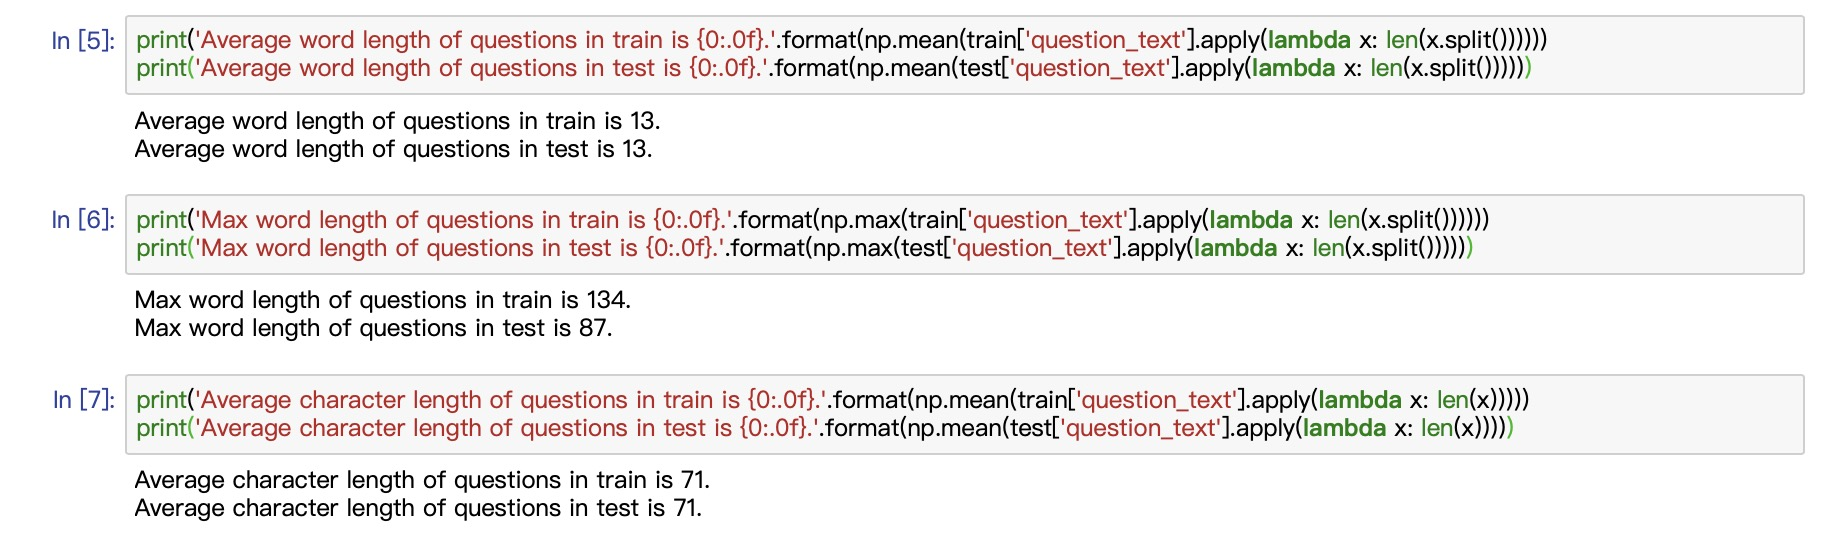
\includegraphics[scale = 0.15]{n2.jpeg}
	\caption{Average length of questions in training dataset and testing dataset}
\end{figure}\\
\noindent We can see that most of the questions are 40 words long or shorter. Let's try having sequence length equal to 71 for now. So in the next model step, we can set the maximum length of words in each sentence is 72.\\
\begin{figure}[h]
	\centering
	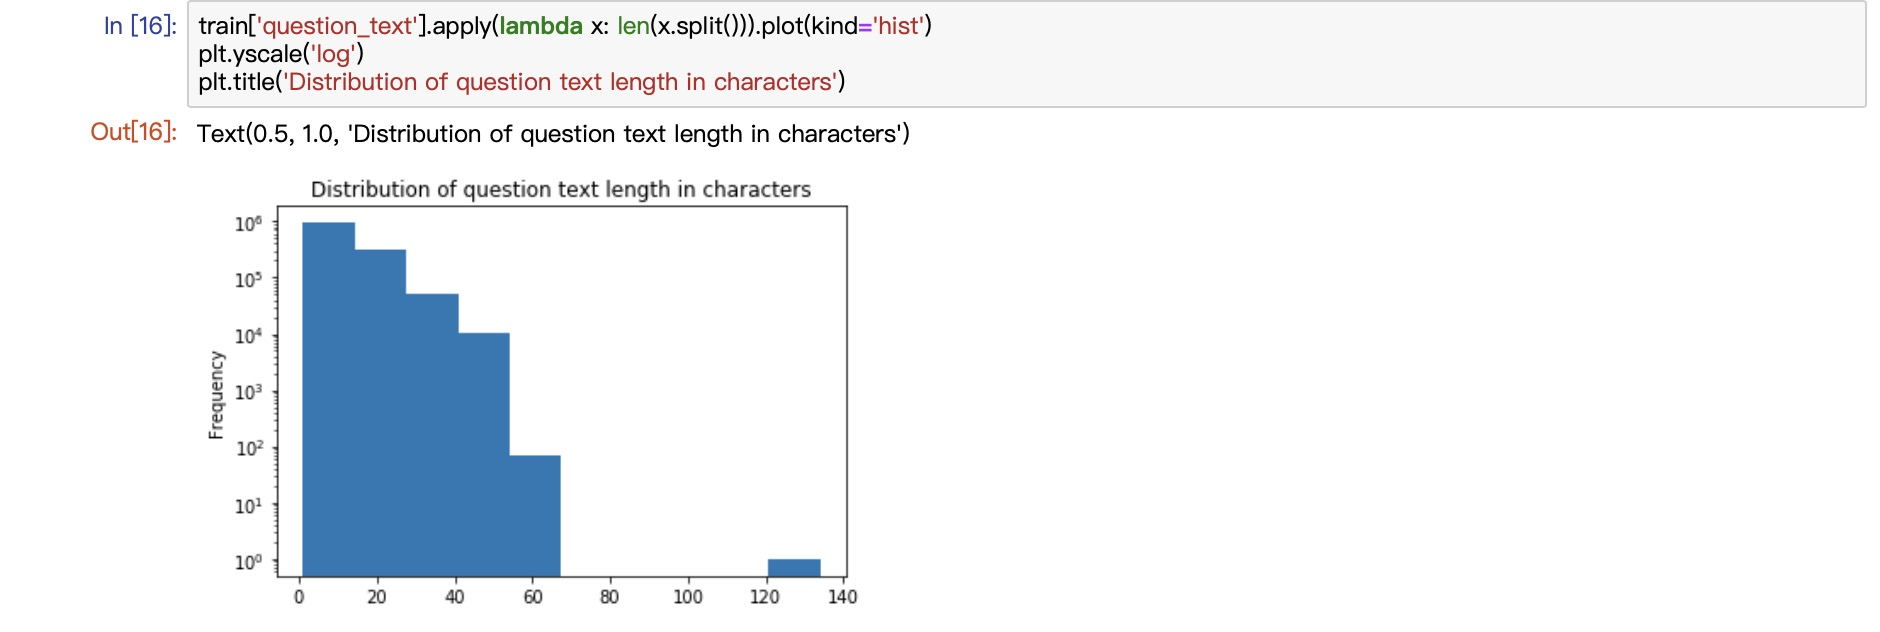
\includegraphics[scale = 0.15]{n3.jpeg}
	\caption{Distribution of question text length in characters}
\end{figure}\\
\noindent Besides, we want to compare words in the wiki dataset and words in the training dataset to detect whether they are good words  or not. In order to avoid spending too much time loading the dataset from the wiki each time when we want to make comparsions, we use "KeyedVectors" library to build a "embeddings\_index". "KeyedVectors" library can help words map to one-dimensional vectors. To the nature of vectors, we can calculate the distance between these vectors to determine are they synonyms.\\
\begin{figure}[h]
	\centering
	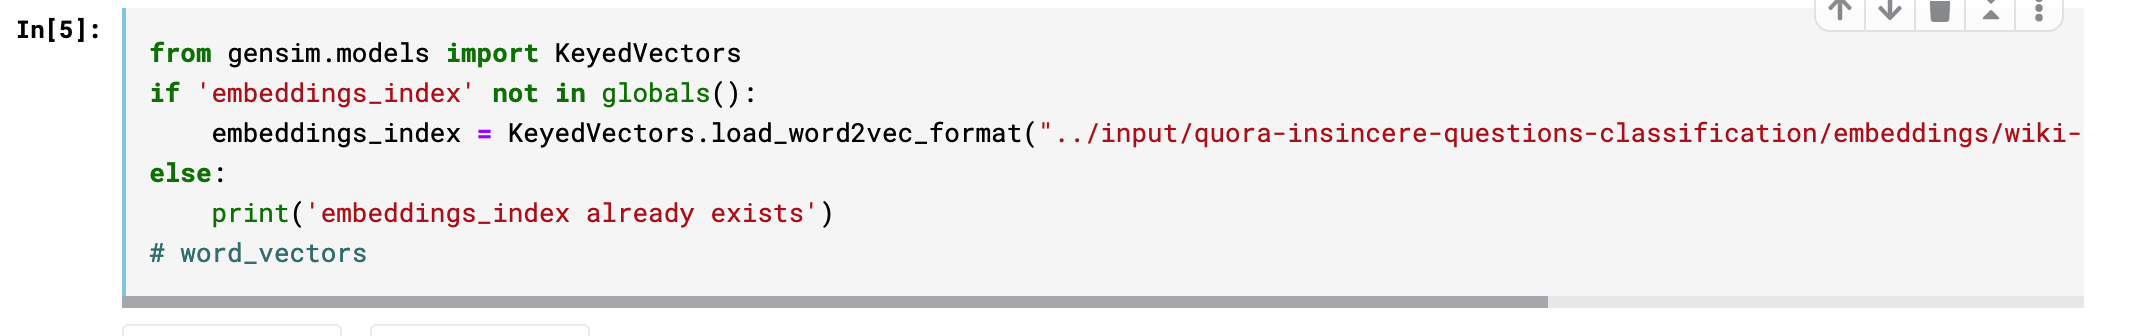
\includegraphics[scale = 0.15]{2.png}
	\caption{Use KeyedVectors library to change words into one-dimensional vector}
\end{figure}\\
\noindent Next question appears in our mind, is that each word in the training dataset can be found according to the "wiki" dataset? So we check the coverage between vocabs in the training dataset's sentences and "wiki" dataset. Surprising find that there around 30.05\%\ percent of words from sentences in the training dataset also show in the "wiki" dataset. 87.66\%\ represent the total frequency of words from the training dataset, which also shows in the "wiki" dataset among the total number of words in the "wiki" dataset and training dataset. This result promote us to doing the next step.\\
\begin{figure}[H]
	\centering
	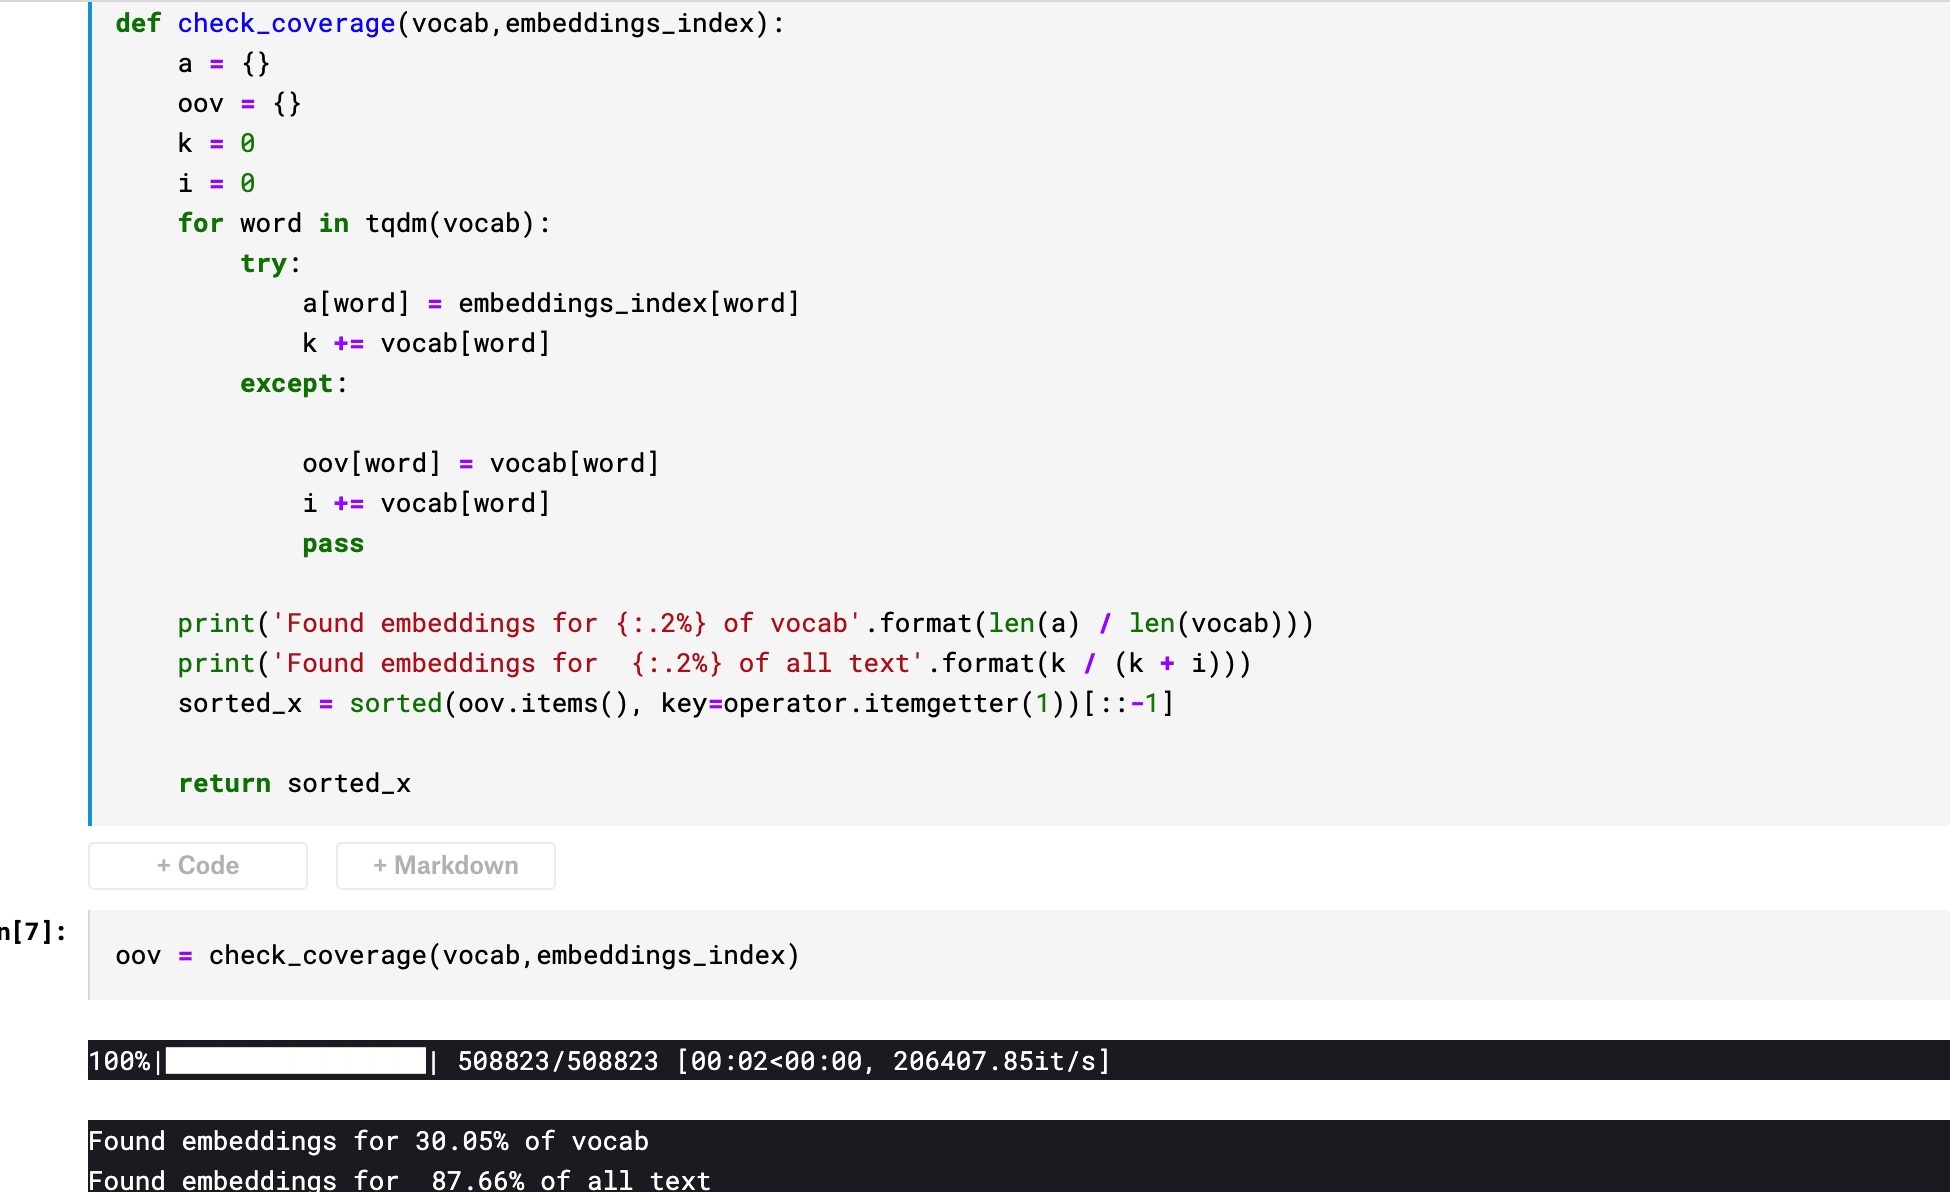
\includegraphics[scale = 0.15]{3.png}
	\caption{Percentage and frequency}
\end{figure}
\noindent We wonder why there is only around 30\%\  of words from the training dataset can be found in the "wiki" dataset. So we print the first 10 rows of " cannot find " words among the "wiki" dataset. It shows that words like "me" and "do" these basic words also cannot find in the "wiki" dataset. The reason is that these words combine together with punctation like " ? " and " ' ". \\
\begin{figure}[h]
	\centering
	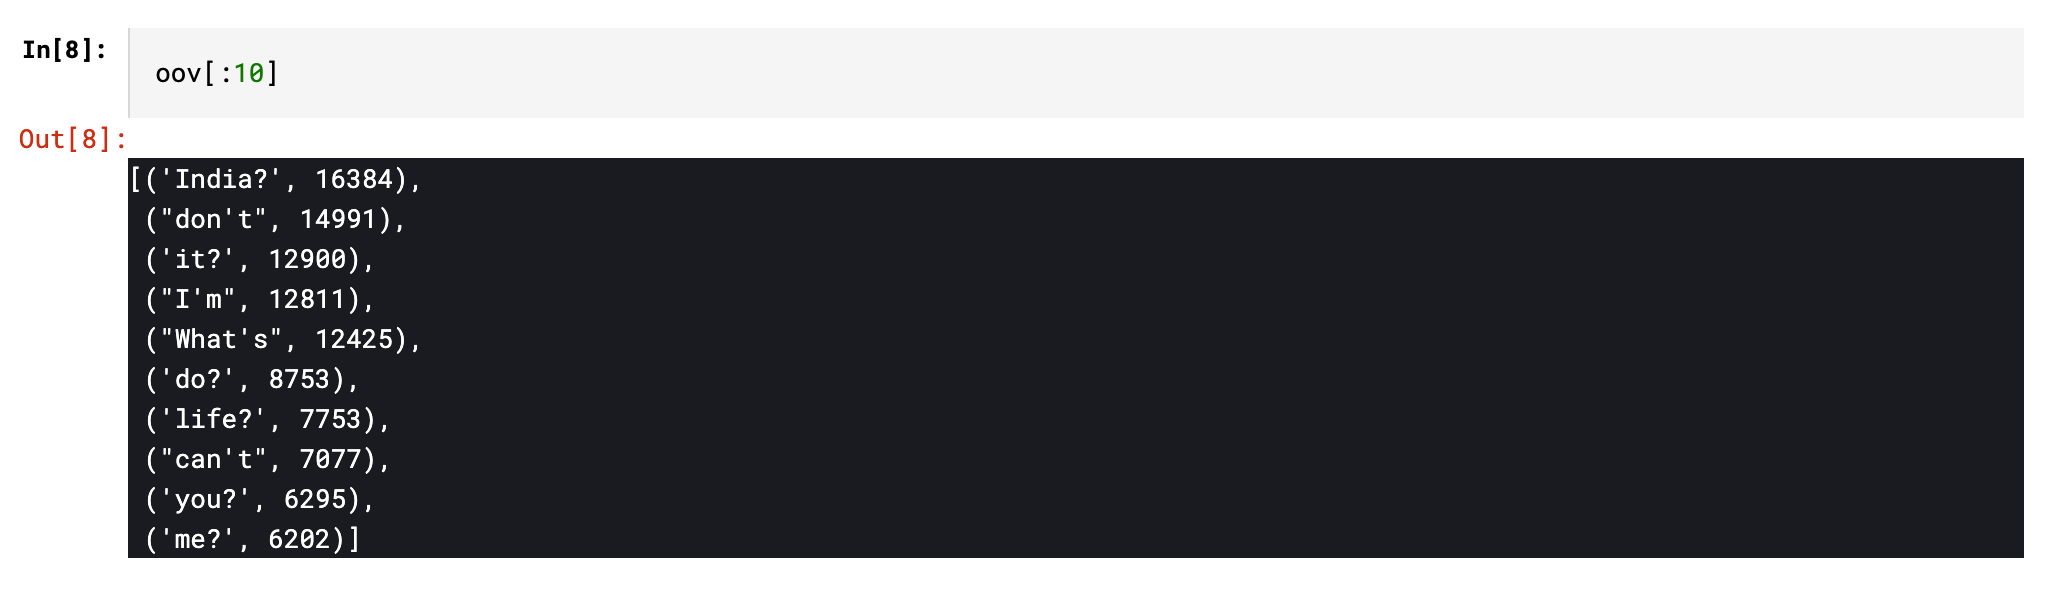
\includegraphics[scale = 0.15]{4.png}
	\caption{First 10 rows of non-found words}
\end{figure}\\
\noindent Continue perusing the provided dataset, we notice that from the "wiki" dataset, it only includes two cases: Single words without punctation and punctation themselves. What's more, the training dataset also includes abbreviations, misspellings and mix of lowercase and uppercase words. Thus, it's necessary to spilt words and punctuations and replace words into correct format to improve our accuracy.\\

\noindent In case, we look up punctation first. We formulate 28 kinds of common punctation and use embeddings\_\ index to find whether it includes in the "wiki" dataset.\\
\begin{figure}[h]
	\centering
	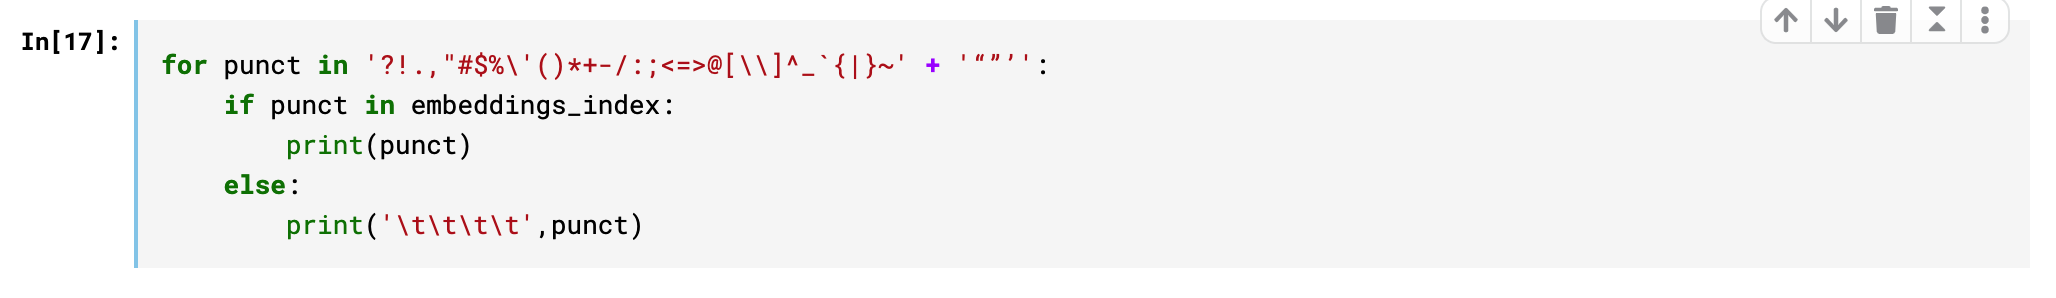
\includegraphics[scale = 0.15]{5.png}
	\caption{Search for punctuations meet our requirement}
\end{figure}\\
\noindent The result is that we found two punctuations " \_\ " and "`" are not in the "wiki" dataset. What's more, we already aware that a word combined with a punctuation will be treated as a cannot find word. To fix this problem, we add spaces on both sides for punctations can be found in "wiki" dataset to separate the punctations and the word. Also, replace the other two cannot find punctuations with spaces.\\
\begin{figure}[H]
	\centering
	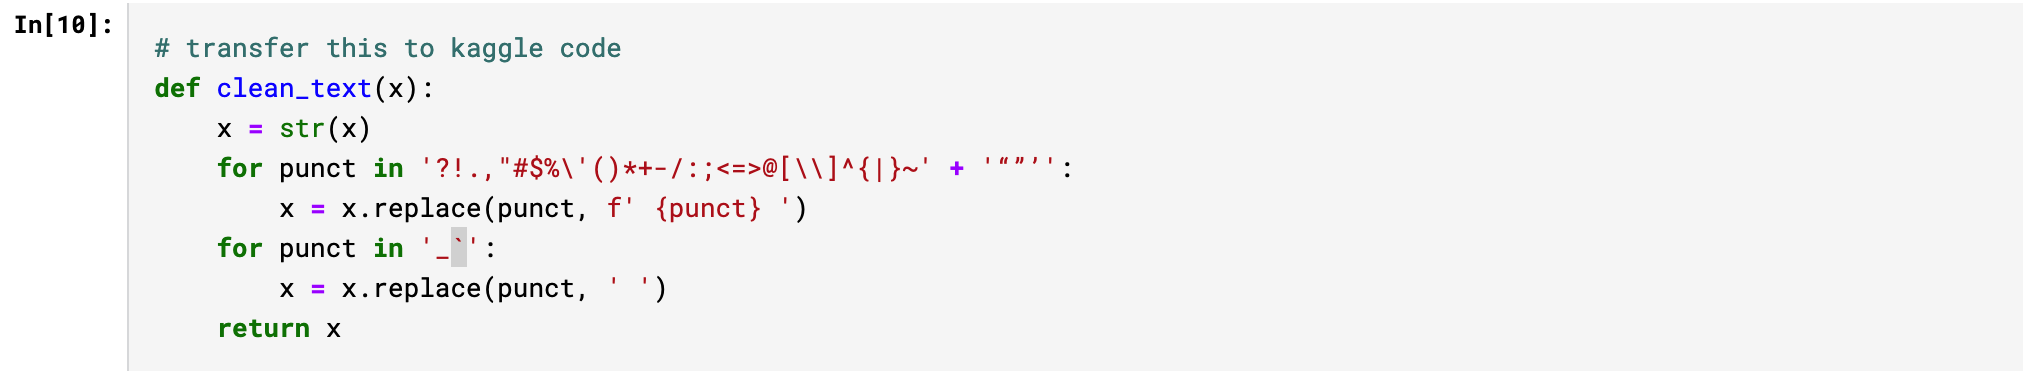
\includegraphics[scale = 0.15]{6.png}
	\caption{Split and replace punctuations}
\end{figure}
\noindent Next step is how to deal with  “cannot find " words among the "wiki" dataset. So our group discuss two  methods to decrease the amount of the word in oov( “cannot find " words).  It is common that netizens often mistyped words or prefer abbreviations for convenience. Therefore, replacing Mistaken spelling words and abbreviated form with correct or appropriate words could increase the ratio of the total number of words in the "wiki" dataset . 
\begin{figure}[H]
	\centering
	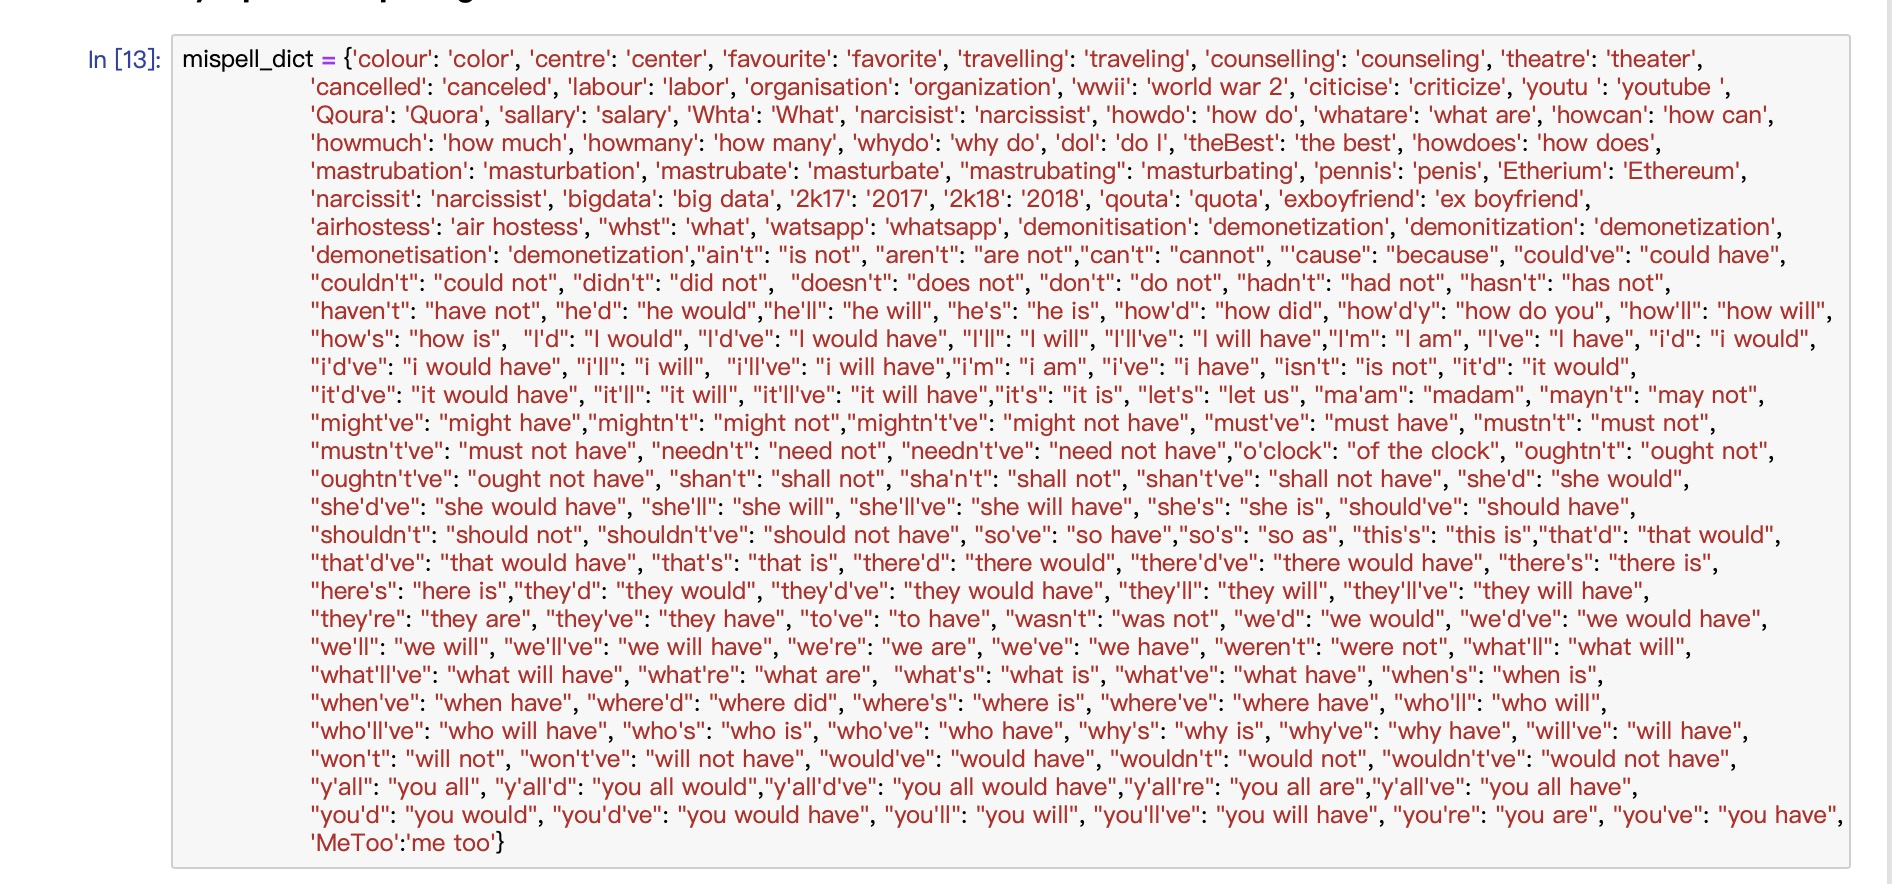
\includegraphics[scale = 0.15]{mis.jpeg}
	\caption{Mistaken spelling and abbrevited words}
\end{figure}
\noindent When we have ruled out the  possibility of mistyping, the length of “cannot find” words is still very high. How can we do?  Is it possible that replace the “unknown” words with words among “wiki” datasets? Based on this assumption, we start to try some special methods. We first sort the 1000 “cannot find”words with high frequencies, and then separately count how many times they appears in good\_sentence and bad\_sentence in terms of labels(0 or 1) in train and test datasets. The percentage of each word able to lead one sentence to be bad(means the corresponding label equals to 1) could generate through the equation r = bad\_sentence/(good\_sentence+bad\_sentence).\\
\begin{figure}[H]
	\centering
	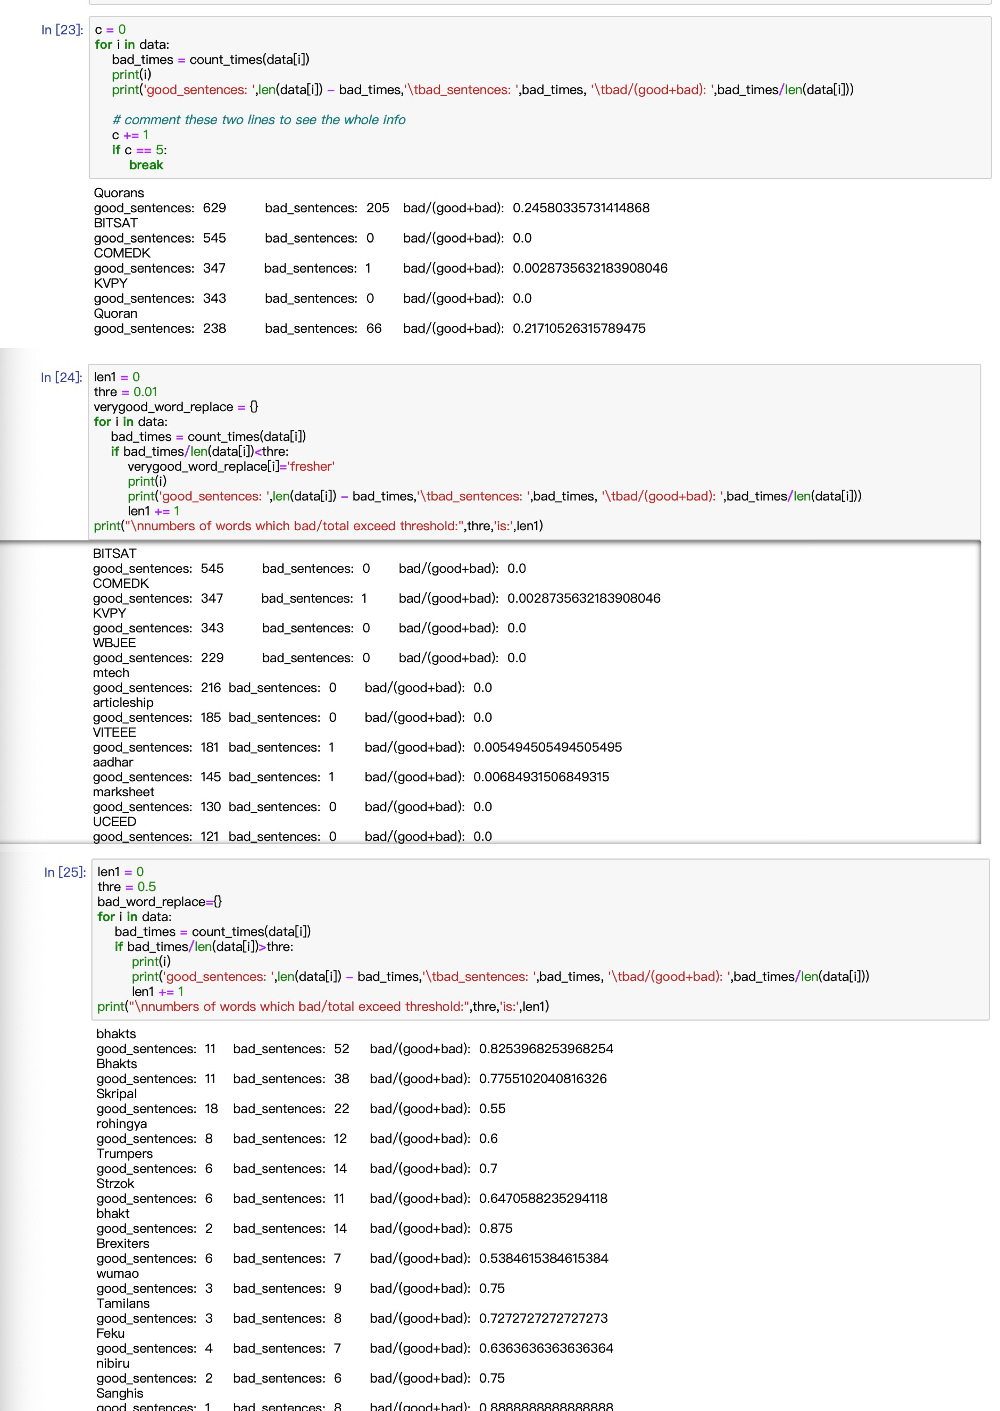
\includegraphics[scale = 0.15]{insert.jpeg}
	\caption{Calculate bad ratio of words that cannot find from wiki dataset}
\end{figure}
\noindent At the same time, select 1000 sentences respectively from good\_sentence and bad\_sentence. And calculate the ratio of each word in these sentences. We set up the threshold less than 0.01 and more than 0.5 in order to get replaceable according to similar ratio values.  
\begin{figure}[h]
	\centering
	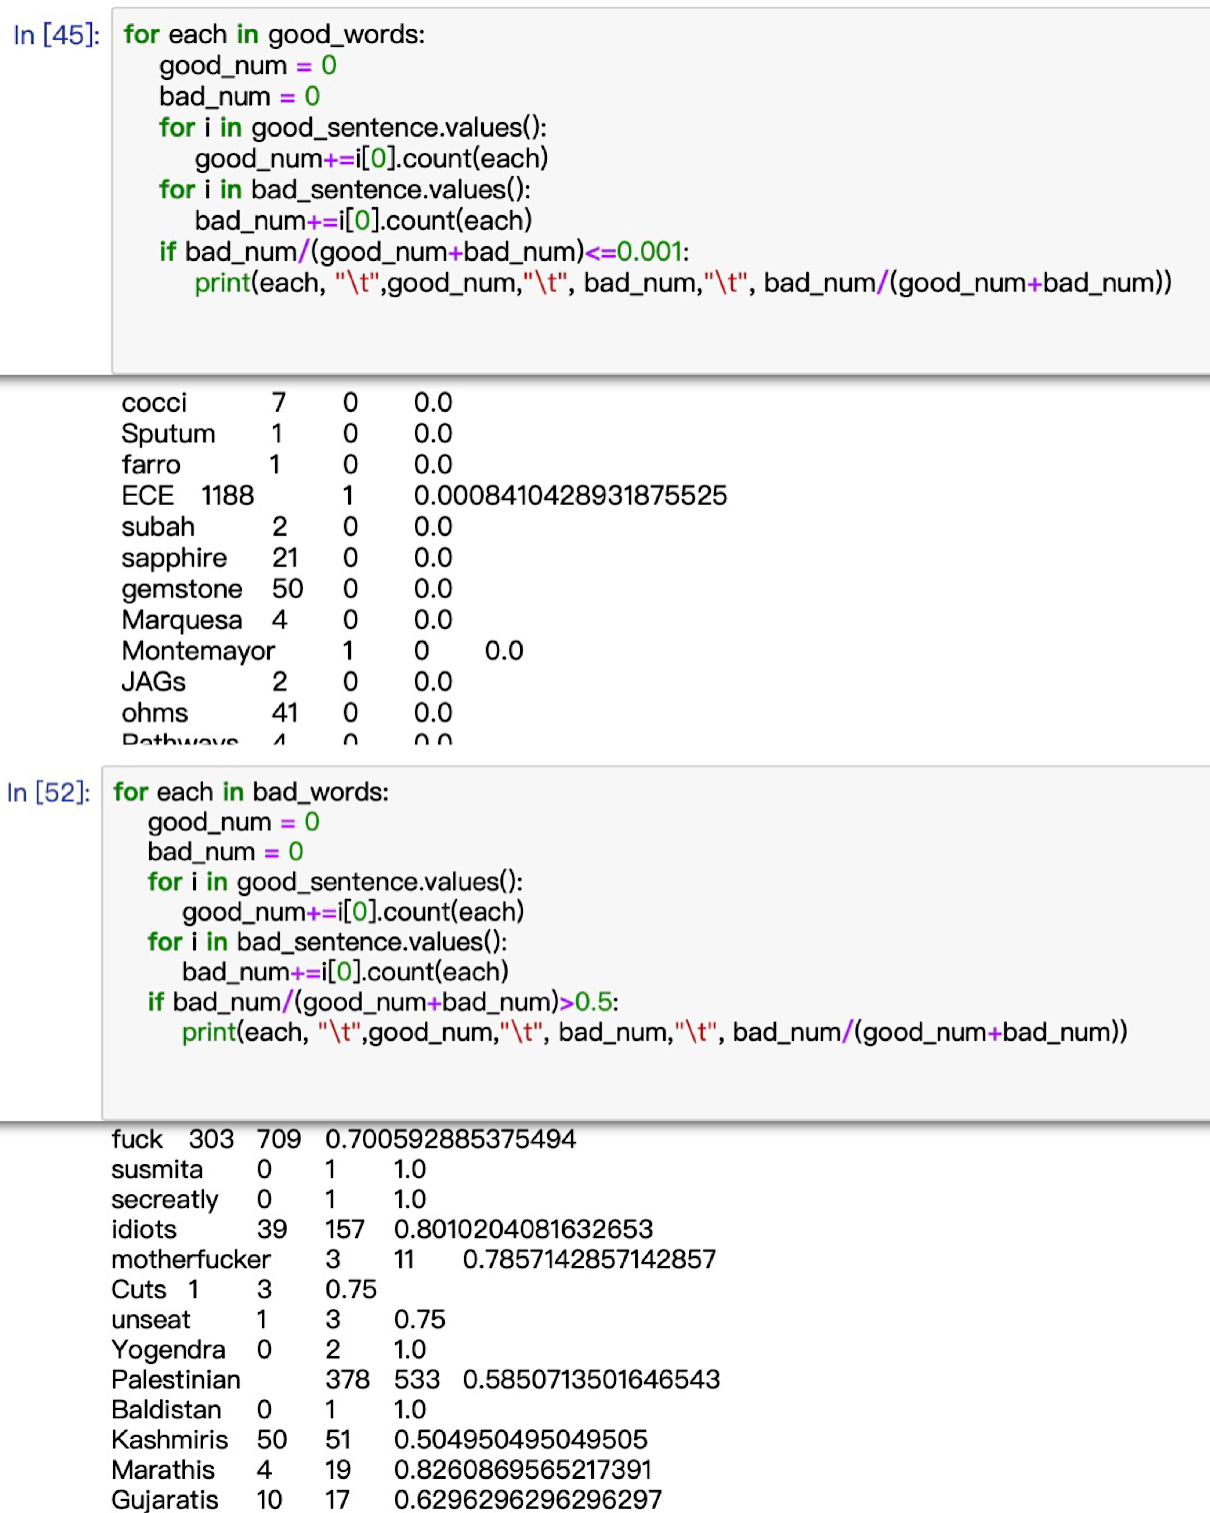
\includegraphics[scale = 0.13]{gb.jpeg}
	\caption{Calculate bad ratio of the replaceable words from good and bad sentences}
\end{figure}\\
\noindent For example, we can see that the ratio of ‘bhakts’ ia about 0.8254, and the word ‘Marathis’ has similar value. As to this situation, it is theoretically feasible to replace ‘bhakts’ with ‘Marathis’. \\

\noindent Therefore, our group implement several methods and then realize  the goal of reducing the length of the list (“cannot find” words). Now the length of the list changes from 81253 to 79883.

\section{ Model Selection}
\noindent In deep learning when we talk about text classification,
the first and most popular model appears in our mind must be RNN model. As we read a sentence, we will not restart from the beginning of the sentence when we meet a new word. Our brain will comprehension from words we have already read and infer the meaning of new words. At this time, our own modules are inspired by Vanilla RNN, LSTM and GRU these three modules. Besides we also make stack and combination from three modules above.
\subsection{Vanilla RNN}
\noindent Recurrent neural networks is not a new topic in deep learning area. Many famous network company as Baidu, Google extensively use this technique with machine translation, speech recognition as well as a number of other tasks. Especially, almost all state of the art outcomes in NLP related tasks are achieved by exploiting RNNs. Before RNN, traditional neuron networks cannot contain persistance, it seems like a corrupt practices. But the occurane of RNN solve this problem.
\begin{figure}[H]
	\centering
	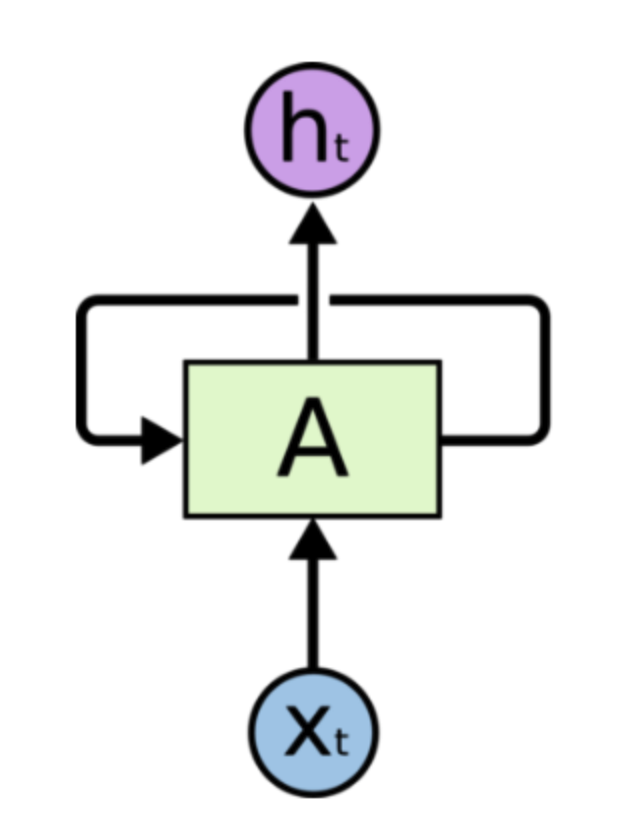
\includegraphics[scale = 0.15]{7.png}
	\caption{Single recurrent neural network model}
\end{figure}
\noindent The recurrent neural networks model is in Fig.7 above. During each time period, each node receives information from the previous node and the process can be represented by a feedback cycle. Fig.8 shows the details of this "feedback" cycle.
\begin{figure}[h]
	\centering
	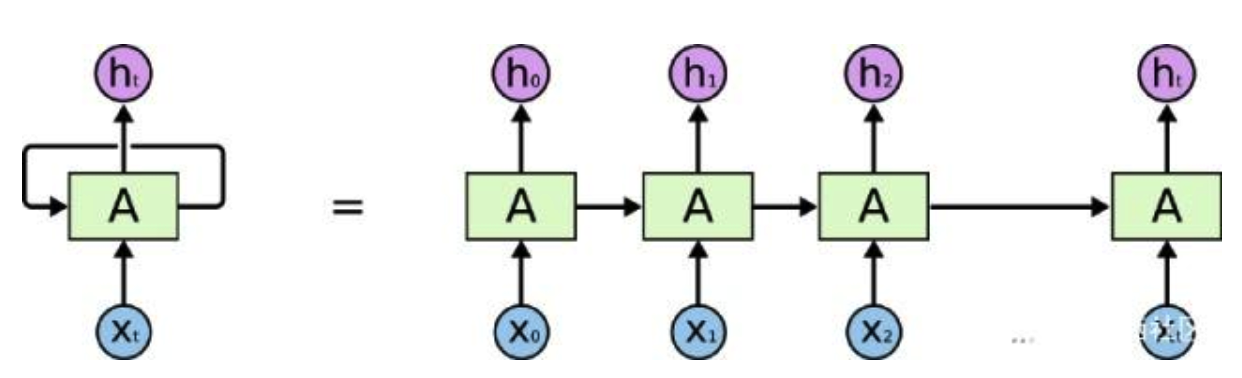
\includegraphics[scale = 0.2]{8.png}
	\caption{How recurrent neural network work}
\end{figure}\\
\noindent In each time process, we pick an input " xi " and output of previous node's output "ai - 1". Calculate them and get the output of the current node " hi ". Same, the output "hi" also provided to the next node as it's input. The cycle will continue running until all time process finish.\\

\subsection{LSTM}
\noindent The defect of RNN is that with the growth of time period, it cannot get effect information from the time period a long time before. As shown in Fig.9, if we want to know more information with "t+1", we probably need to realize the meaning from "0" and "1" in the time process. Due to the long distance, the model learns from "0" and "1" cannot be expressed to the node with " t+1 ". As far as we can see, RNN can only memorize the short information sequence.
\begin{figure}[h]
	\centering
	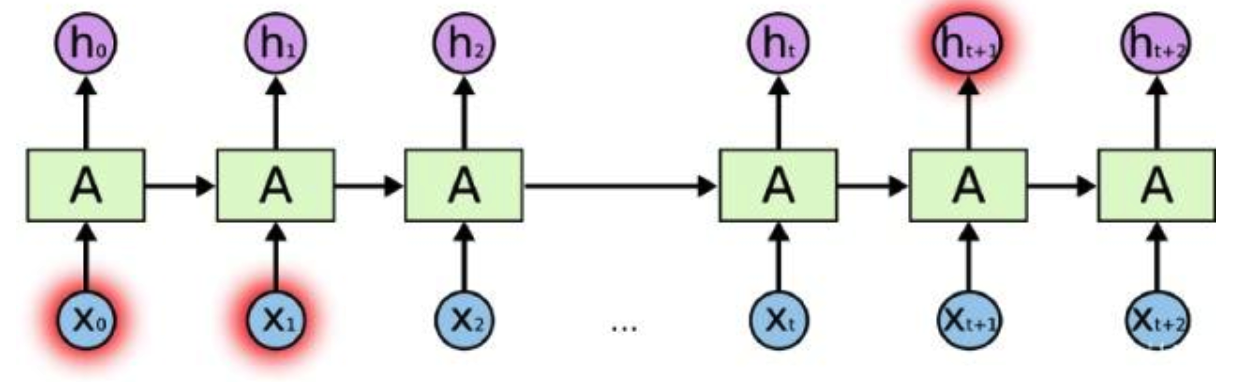
\includegraphics[scale = 0.15]{9.png}
	\caption{RNN cannot get information with long period before}
\end{figure}\\
\noindent As a result LSTM networks came. LSTM is not a totally new module, it's a kind of evolution from RNN module. In order to keep and transfer information for a long period of time is the default behavior of these networks. Comparing with the structure, both LSTM and RNNs have a chain like shape. But the repeating module from two models are quite different. The original repeating module of RNNs only has a single tanh layer, but LSTM module contains four interacting layers.
\begin{figure}[H]
	\centering
	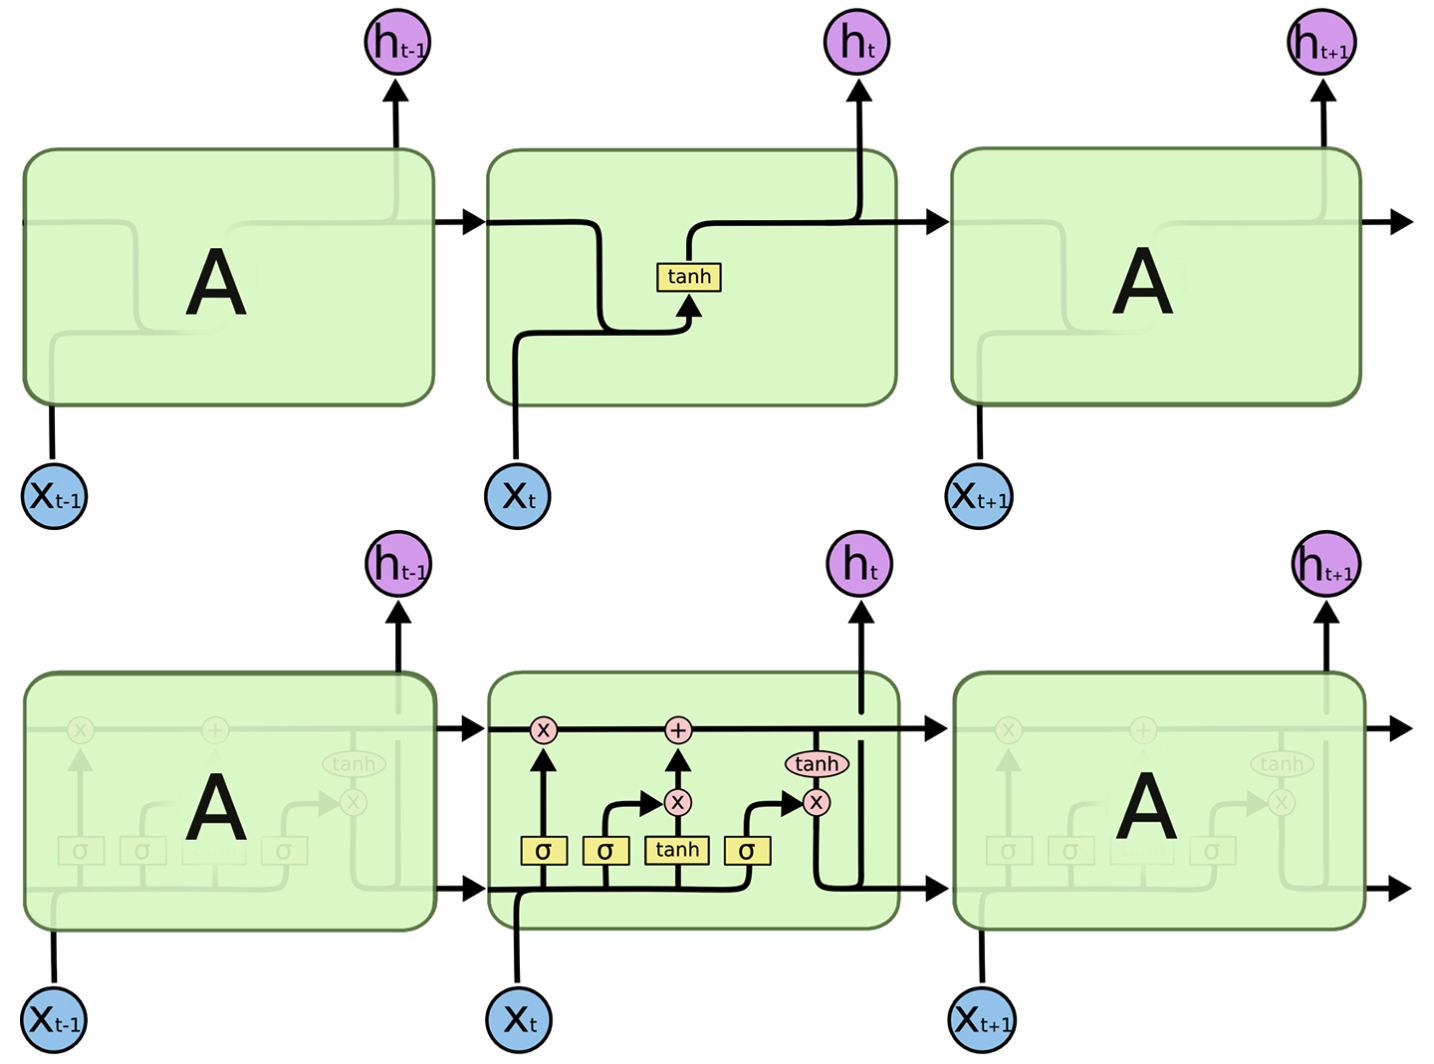
\includegraphics[scale = 0.15]{10.png}
	\caption{RNNs module structure vs. LSTM module structure}
\end{figure}
\noindent The key point of LSTM is that it includes a "coveyor belt" within the module structure. Information will transfer on this "conveyor belt" and only few linear interaction can prevent the loss of information. There are three different gates collaborate together : "Foget", "Refresh" and "Output". \\
\subsection{GRU}
\noindent When we train the LSTM module, we find that although the result comes from LSTM is much better than vallina RNN module, but the time cost is also higher. In that case, we notice that LSTM module has a variant module "GRU".
\begin{figure}[H]
	\centering
	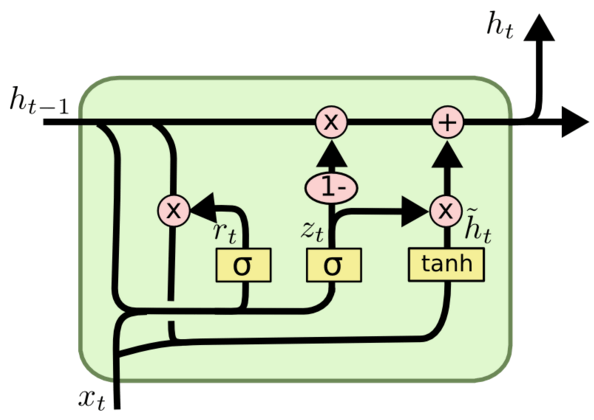
\includegraphics[scale = 0.15]{11.png}
	\caption{GRU module}
\end{figure}
\noindent From Fig.11, it's obvious that inside of the GRU module, there are only two gates named "Refresh" and " Reset" instead of three gates in the LSTM module. The "Refresh" gate decides how much previous information we need to go through and the "Reset" gate decides how much former information the module should discard.\\

\noindent In theoretical, because of the decrease of parameters in the GRU module, the computational efficiency of GRU will higher than LSTM. \\

\section{ Implementation}
\subsection{Embedding}
\noindent Before we feed the training data into our model, the first thing after cleaning the data is to transfer string type data to vectors. The dictionary we use to convert string is wiki-news-300d-1M.vec which supplied by Kaggle. Wiki-news-300d-1M is a dictionary with one million words(including punctuations and numbers). And each key is one word, each value is a 1-dimension  word vector with 300 numbers.\\

\noindent For the words in training data which can  be found in wiki-news-dictionary, we replace them with vectors. For those can’t be found in wiki-news-dictionary and also escaped from our preprocessing, we initialize them with a random vector which is based on the distribution of the words in text.\\
\begin{figure}[h]
	\centering
	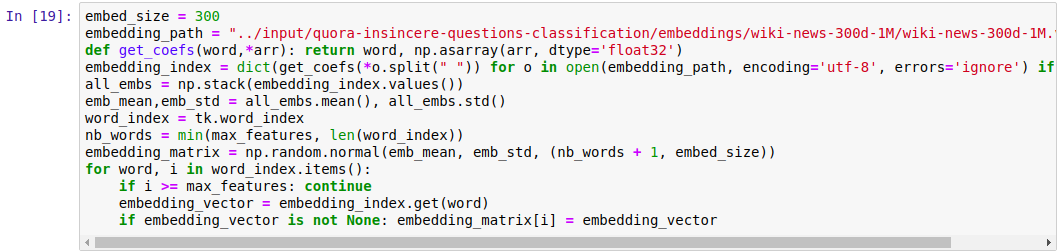
\includegraphics[scale = 0.2]{41.png}
	\caption{Initialize training dataset with random vector}
\end{figure}\\
\noindent After all these steps, the data is ready to be fed into our models.\\

\subsection{LSTM}
\subsubsection{One layer LSTM}
\begin{figure}[h]
	\centering
	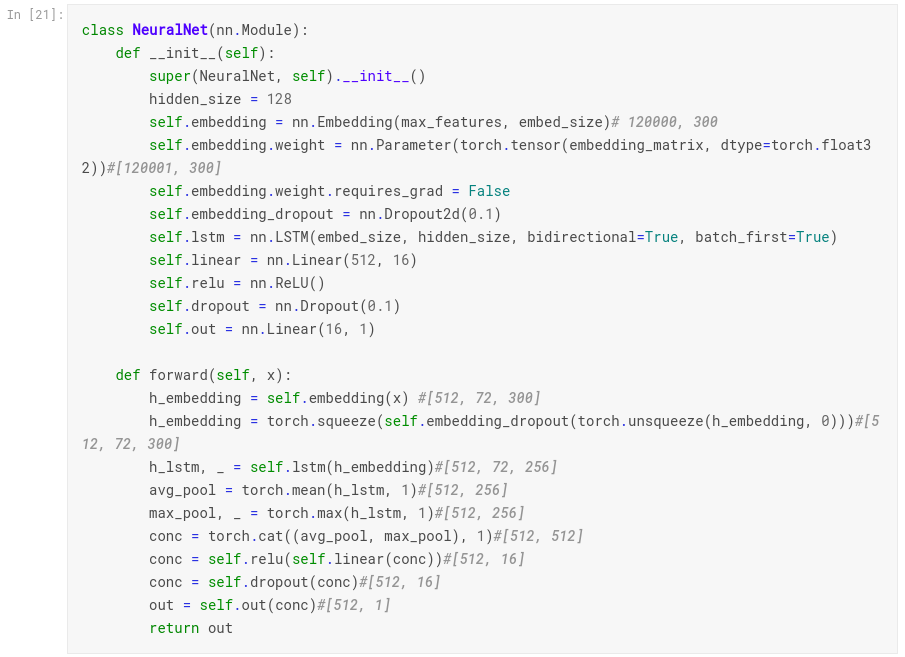
\includegraphics[scale = 0.2]{42.png}
	\caption{One layer LSTM model}
\end{figure}
\noindent First model is just a simple one-layer LSTM model, after going through the LSTM layer, the output of that layer goes through two separate pooling layers in order to obtain information as much as possible. Then we concate the two outputs of the pooling layers and put it into an activation layer and then dropout followed by a linear layer.\\

\noindent There’s only one hyperparameter we adjust in this project- number of epochs. In order to save time, we first tried 5, 7, 10 epochs to train our raw data without replacing misspelling words. The result is shown in Fig.20.\\
\begin{figure}[H]
	\centering
	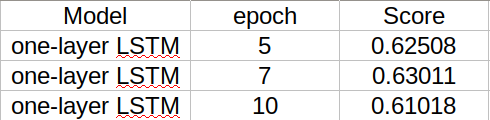
\includegraphics[scale = 0.2]{421.png}
	\caption{Different epochs with one-layer LSTM}
\end{figure}
\noindent Obviously, 7-epoch LSTM has the highest score. And this is the reason that we choose seven epochs to train our following models.
With preprocessed data fed into model, we get the result shown below. And the average time training one epoch is at around 75s.
\begin{figure}[H]
	\centering
	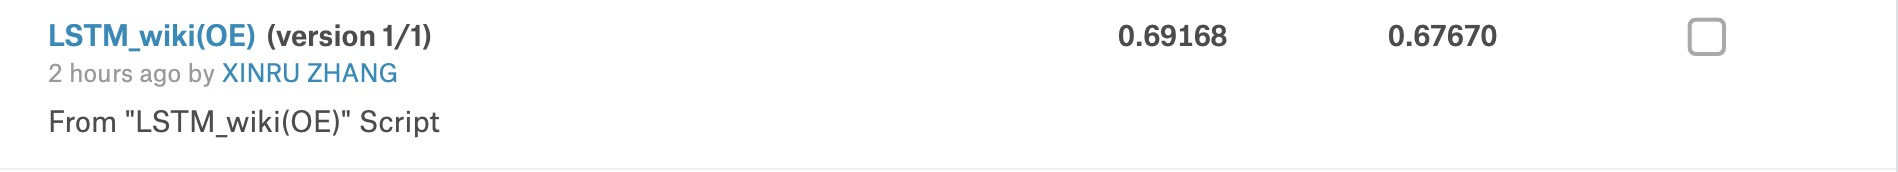
\includegraphics[scale = 0.2]{4211.jpeg}
	\caption{One-layer LSTM(7 epoch)
	}
\end{figure}
\begin{figure}[H]
	\centering
	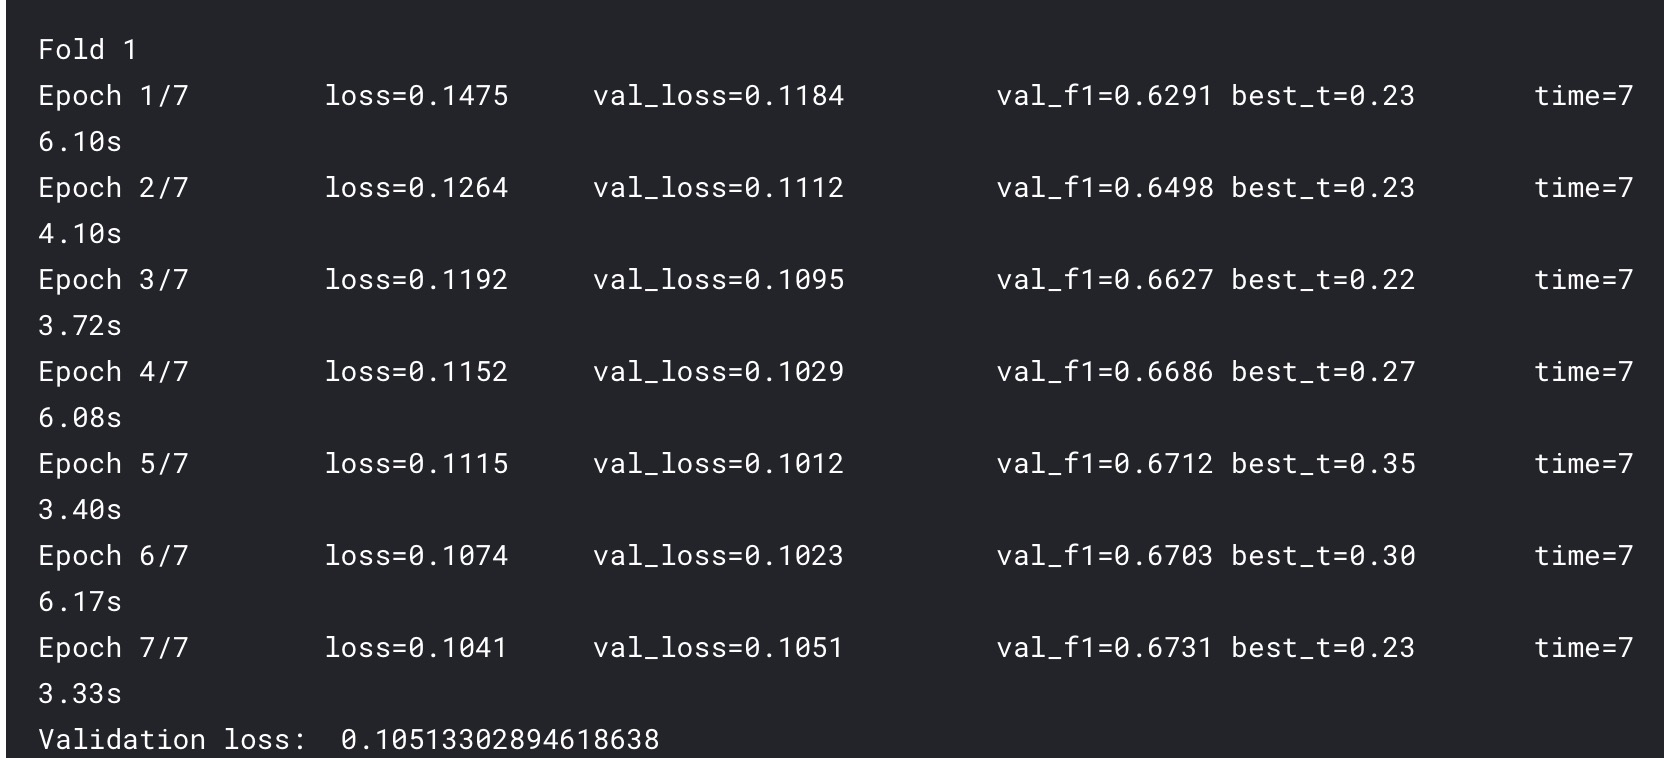
\includegraphics[scale = 0.2]{4212.jpeg}
	\caption{Part training result. Average training time consuming for one epoch is around 75 second
	}
\end{figure}
\subsubsection{ Two and three layers LSTM}
\noindent We also tried two -layer and three-layer LSTM models with seven epochs. With raw data, the two-layer LSTM got 0.63068 on final result which performs better than one-layer LSTM but the three-layer LSTM got 0.62601 which is worse than the two-layer LSTM model. The reason may be that three layers model is too much for the training data, the model got overfitting on the data.\\
\begin{figure}[H]
	\centering
	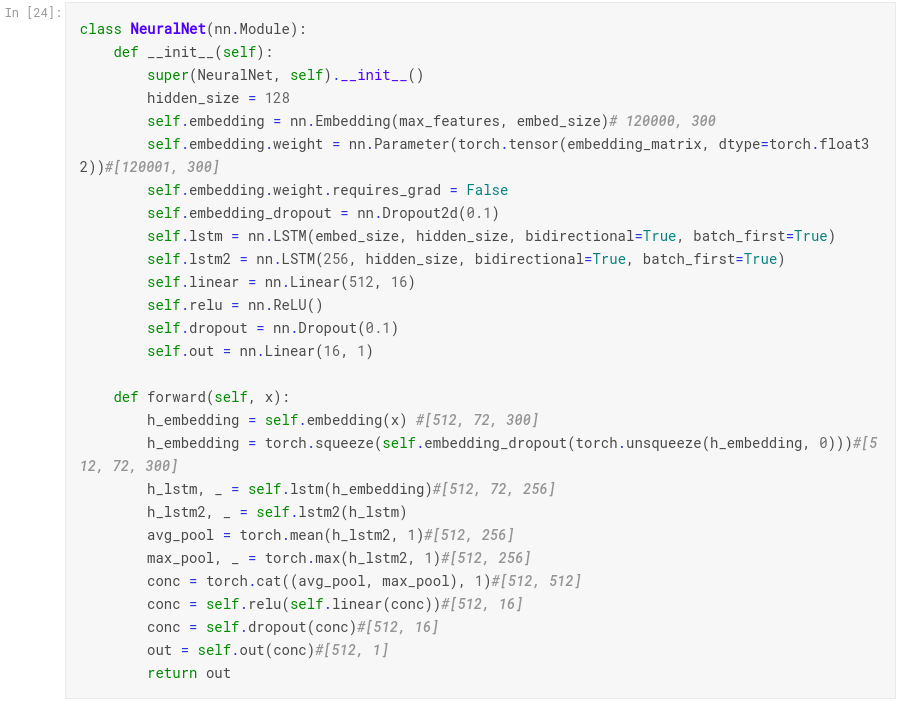
\includegraphics[scale = 0.2]{422.png}
	\caption{Two-layer LSTM}
\end{figure}
\noindent After feeding preprocessed data to two-layer LSTM model, we got 0.68421 which is the highest score among all the LSTM models.\\
	\begin{figure}[H]
		\centering
		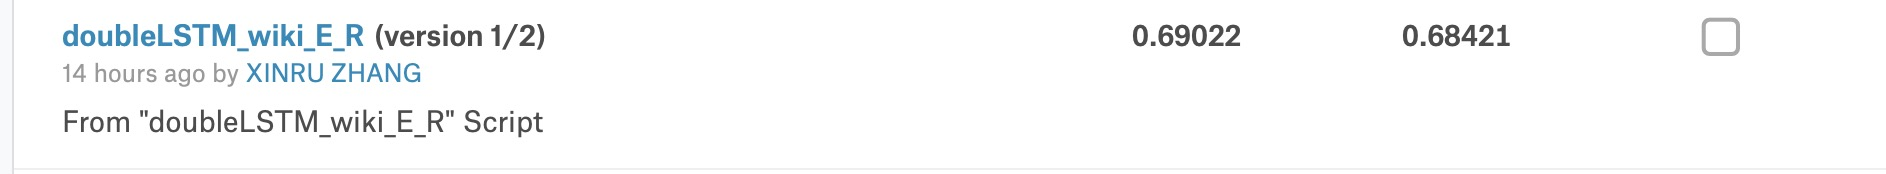
\includegraphics[scale = 0.2]{4221.jpeg}
		\caption{ Two-layer LSTM score }
	\end{figure}
\subsection{Simple GRU}
\noindent Simply replacing nn.LSTM with nn.GRU give us one-layer GRU model. Compared to one-layer LSTM, we got a higher score(0.68206) and less training time(at around 44s).\\
	\begin{figure}[H]
	\centering
	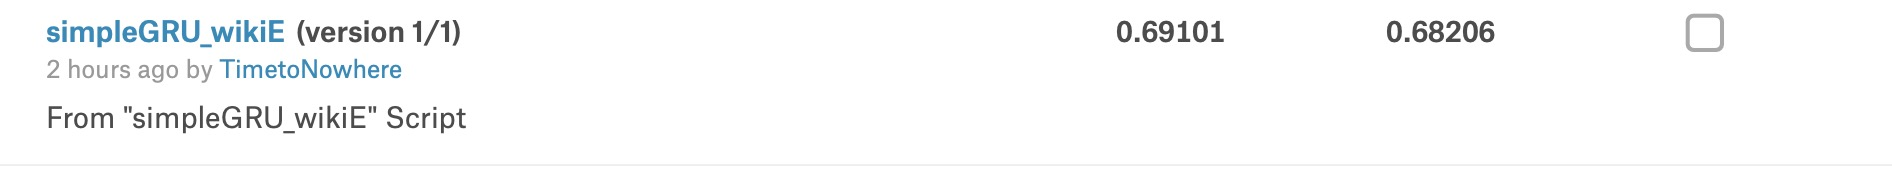
\includegraphics[scale = 0.2]{431.jpeg}
	\caption{ One-layer GRU socre}
\end{figure}
\begin{figure}[H]
	\centering
	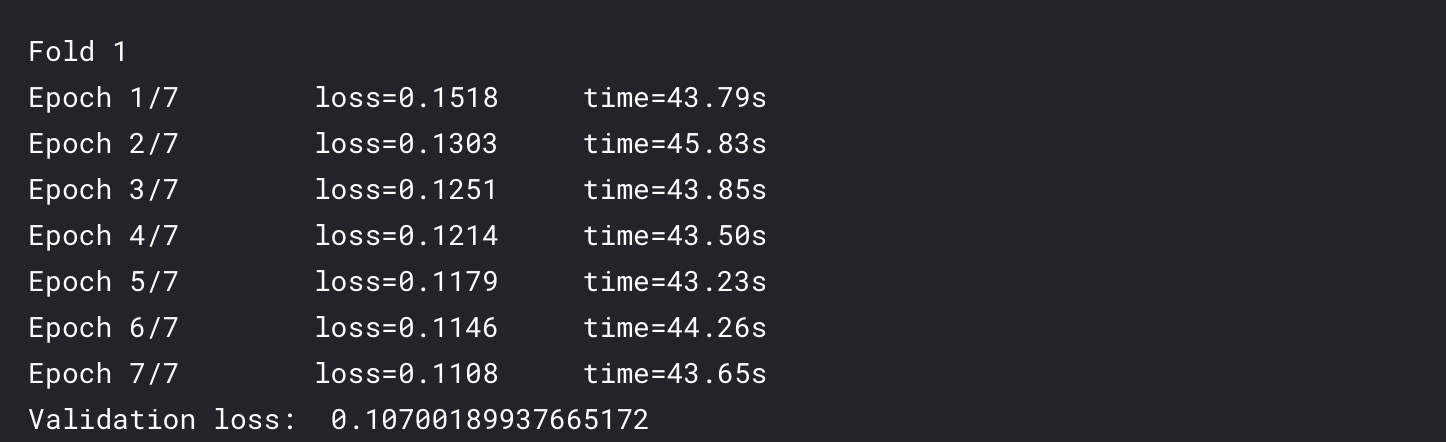
\includegraphics[scale = 0.2]{432.jpeg}
	\caption{Part training result. Average training time consuming for one epoch is around 44 second}
\end{figure}
	
\section*{Reference}
\small

\noindent [1] Goodfellow, I.\ \& Bengio, Y.\ \& Courville, A.\ (2016) Deep Learning. {\it Modern Practical Deep Networks},
pp.\ 367--403. Cambridge, MA: MIT Press.\\

\noindent[2] Supervise, ly., (2017) Towards Data Science:
{\it Evolution: from vanilla RNN to LSTM \& GRU.} [online]Available at <https://towardsdatascience.com/lecture-evolution-from-vanilla-rnn-to-gru-lstms> (02/12/2019 12:14)\\

\noindent[3] Hoffman, G.(2018). {\it Introduction to LSTMs with Pytorch.} O'Reilly AI Newsletter, 54, 66-80.\\

\noindent[4] Adrianna, X., (2017) More or Less?:{\it Talking about the difference with LSTM and GRU.}
[online]Available at <https://blog.csdn.net/u012223913/article/details/77724621> (30/11/2019 17:34)\\

\noindent[5]  Hao, L., (2018) Talking about Nature Language Processing: {\it
Word Embedding}. [online]Available at <https://blog.csdn.net/L\_R\_H000/article/details/81320286> (02/12/2019 12:44)\\

\noindent[6]  Xiaozhou, Y. \ \& Feifei, T.\ \& Rongzhi, Q. (2016). {\it Improvement of activation function in recurrent neuron network.} Journal of computer and modernization,12, 14-27.\\
\end{document}
